\section{Introduction}\label{sec:intro}
In this project we are given some basic volume visualization application and will implement several additional features in order to enhance this application. To be able to clearly explain the added functionality, we start by shortly describing the initial functioning of the application.

Technically speaking, it could be argued whether the initial application is even a real raycaster, as it simply takes a slice through the data, and projects this data onto the viewing window (see figure \ref{fig:raycaster0}). The slice is defined in such a way that it always goes exactly through the center of the volume bounding box, and is oriented perpendicular to the view vector \texttt{viewVec}. As the view vector is again perpendicular to the view window, the slice is always parallel to the view window. The width and height of the slice are both defined by the diagonal of the bounding box. This is an obvious choice, because this is the smallest dimension that ensures that no data can ever lie outside of the slice area.

When looking at the code of the initial application, we observe that all of the above functionality is realized by a function called \texttt{slicer()}, which uses a simple nested for-loop to walk along all the pixels of the view window in horizontal and vertical direction. For each pixel, the value is then determined as follows. First we cast a ray from that pixel, parallel to the view vector. We then determine the $x$-, $y$- and $z$-coordinate of the intersection of this ray with the slice plane.
This is done using two additional vectors \texttt{uVec} and \texttt{vVec} that are defined by a plane through the origin, perpendicular to the view vector.
Once the coordinates are determined, they are passed on to a function called \texttt{getVoxel()}. This function then rounds the three coordinate values in order to obtain the voxel that is closest to the received coordinate (i.e. the nearest neighbor voxel). The value of this voxel is then returned to the slicer function, and passed on to the function \texttt{tFunc.getColor()}, obtains the correct color for the voxel value that was returned by \texttt{getVoxel()}. This color is finally converted into an ARGB color and drawn onto the view window.

\begin{figure}[h!]
    \centering
    \captionsetup{justification=centering,margin=0.5cm}
    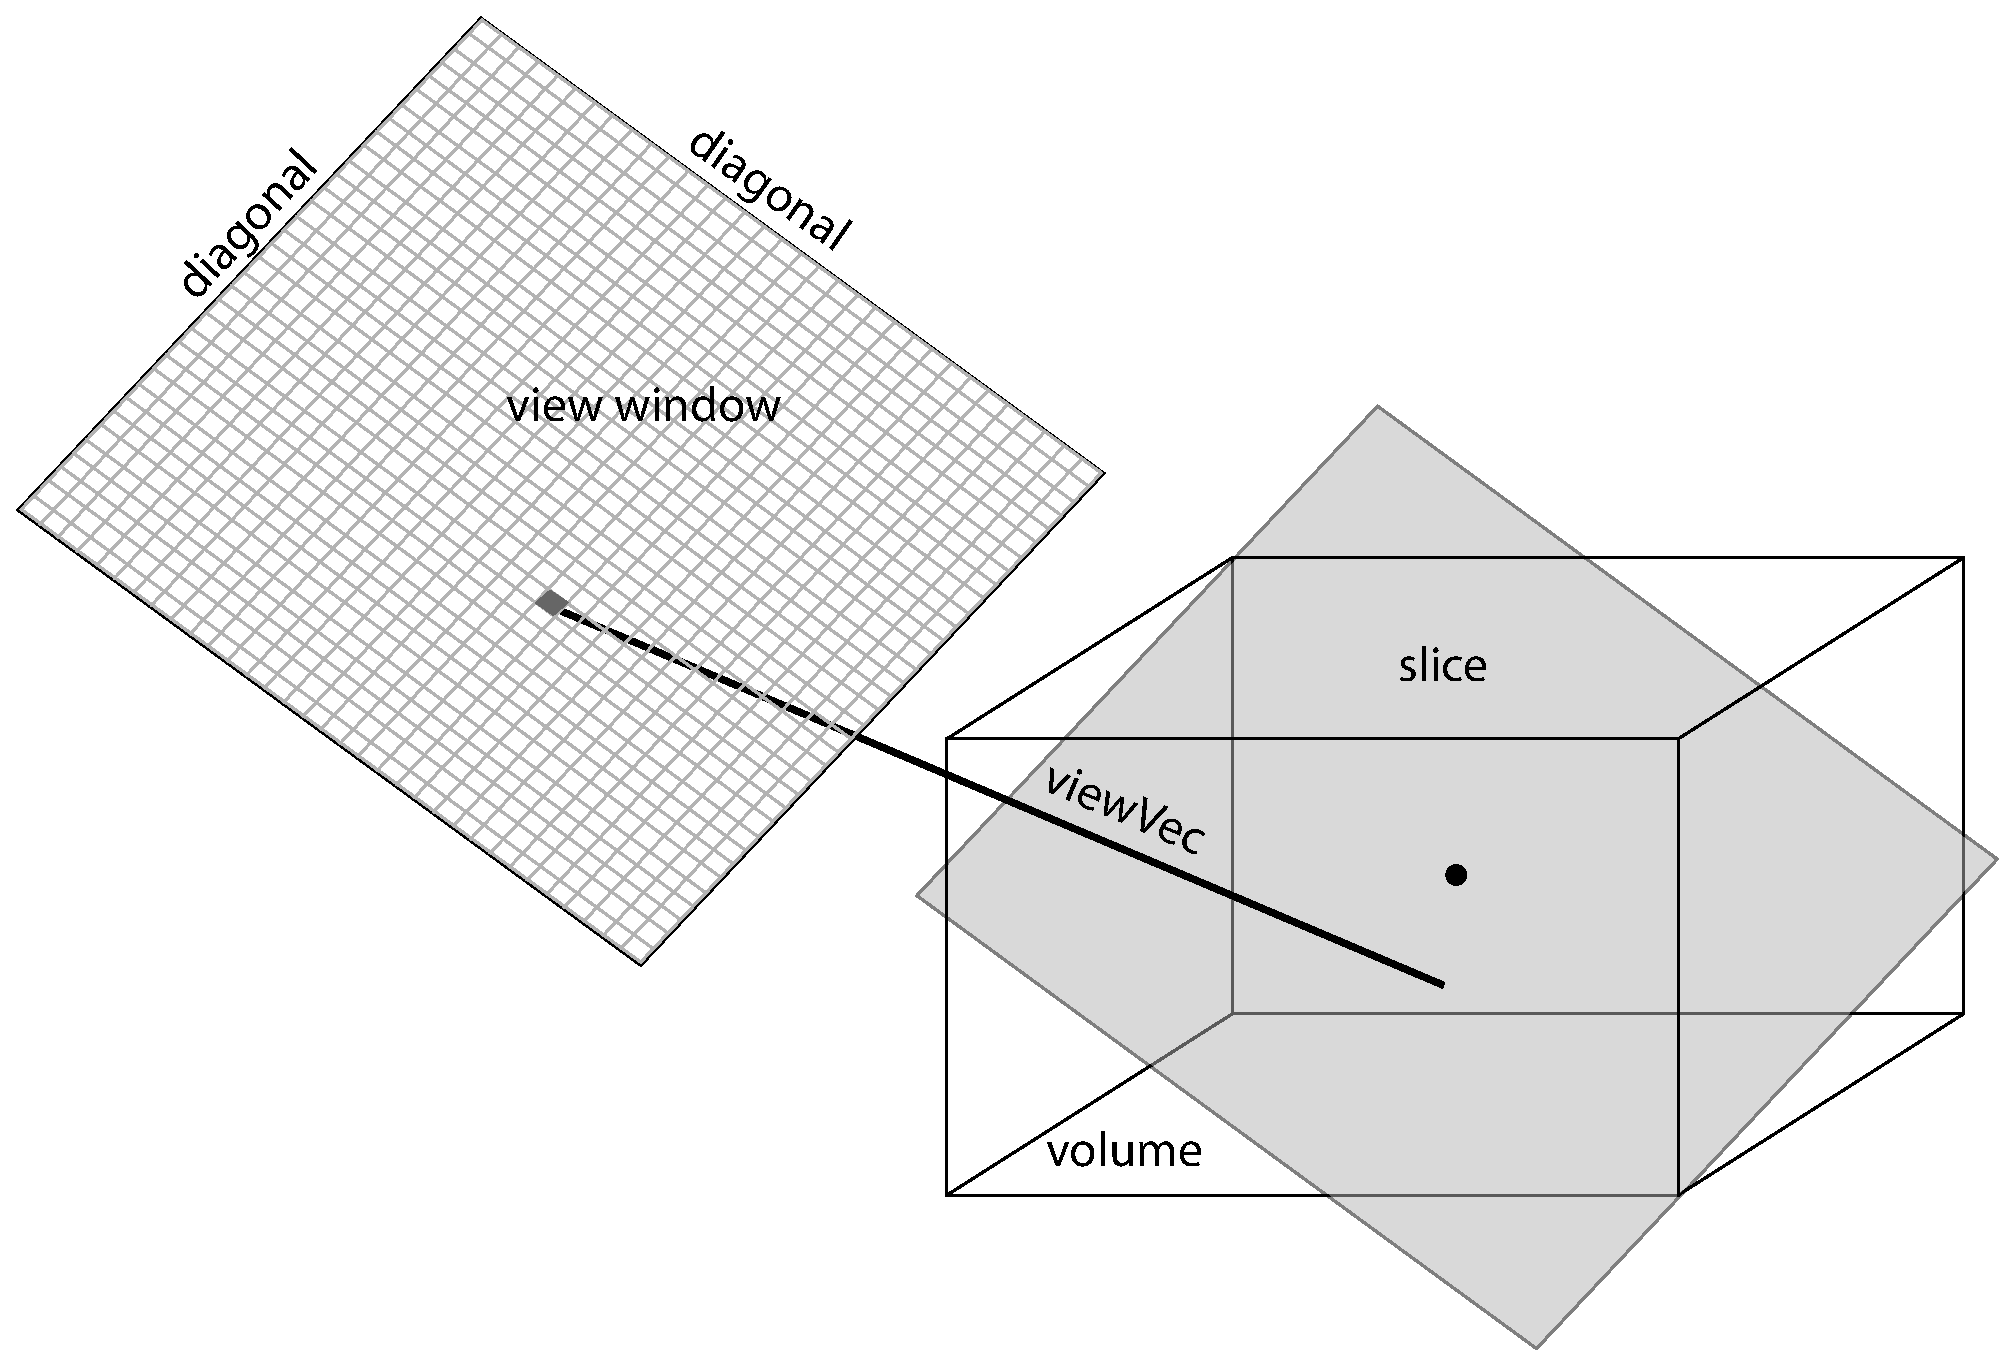
\includegraphics[width=0.8\textwidth]{img/raycaster0.pdf}
    \caption{The initial raycaster application: only a slice of the data within the volume is taken and projected onto the image (screen pixels)}
    \label{fig:raycaster0}
\end{figure}

\newpage

With this application as a starting point, we devote the upcoming sections to explaining the additional features that were implemented. We start in section \ref{sec:mip} with the implementation of a Maximum Intensity Projection method. We furthermore adjust the interpolation technique for the points on a casted ray from a nearest neighbor interpolation to a tri-linear one. Because the implementation of a MIP greatly reduces the performance of the application, we present several performance enhancement methods in section \ref{subsec:perf_enh}. In section \ref{sec:compositing} we present an alternative implementation for the MIP, namely compositing. Section \ref{sec:opacity} finally describes how we implemented gradient-based opacity weighting. For this implementation we used the compositing renderer as the basis and extended it with gradient-based opacity weighting. In subsection \ref{subsec:opacity_compare} the results are compared with the original compositing renderer.
